Laser sind in der Lage Licht mit einer besonders hohen Intensität zu erzeugen. Der Lichtstrahl ist dabei sehr stark fokussiert,
die elektromagnetischen Wellen besitzen die gleiche Frequenz und sind kohärent zueinander. Die Prozesse, die zur
Erzeugung des Laserlichts führen, finden im Wesentlichen in drei verschiedenen Komponenten des Lasers statt.

\begin{figure}
\centering
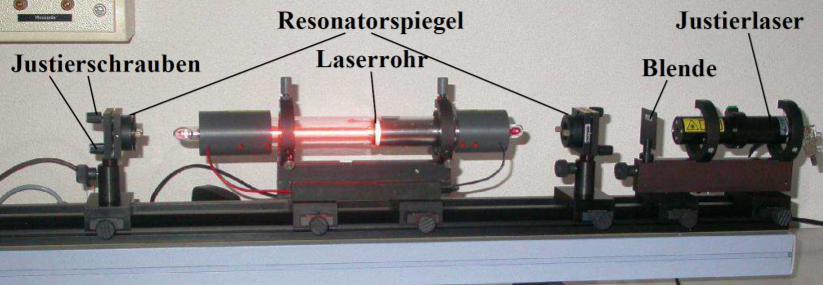
\includegraphics[width=\textwidth]{laseraufbau.png}
\caption{Aufbau eines He-Ne-Lasers.\cite[3]{anleitung}}
\label{fig:laseraufbau}
\end{figure}

\subsection{Der Resonator}

Der Resonator besteht aus zwei Spiegeln, zwischen denen sich ein Glasrohr befindet. Dieses ist mit einem Helium-Neon-Gasgemisch
gefüllt. Die Spiegel sind dabei hochreflektierend, lassen jedoch auch einen kleinen Teil des Lichtes hindurch, sodass das
Laserlicht aus dem Resonator austreten kann. Sie können unterschiedliche Krümmungsradien haben (konkav oder plan-parallel).

Im Resonator bilden sich nur unter bestimmten Voraussetzungen stehende Wellen aus, die dann verstärkt werden können.
Andere Wellen werden aufgrund destruktiver Interferenzen stark abgeschwächt. Nur wenn die Länge des Resonators durch ein
Vielfaches der halben Wellenlänge teilbar ist, überlagern sich die Wellen auf optimale Weise und das Licht wird gut verstärkt.

Links und rechts des Resonators sind außerdem noch Brewsterfenster angebracht, die dafür sorgen dass das emittierte Licht
parallel-polarisiert ist. Die Fenster stehen im Brewster-Winkel zur optischen Achse, sodass senkrecht-polarisiertes
Licht herausgefiltert und das Licht in Ausbreitungsrichtung verstärkt wird.

Ein Resonator gilt als stabil, wenn seine Verluste möglichst gering sind und die Verstärkung des Lichts gut funktionniert.
Die Bedingung für Stabilität ist dabei durch den Stabilitätsparameter $g_1g_2$ gegeben. Er sollte zwischen 0 und 1 liegen.

\begin{equation}
  g_1g_2 = \biggl(1-\frac{L}{R_1}\biggr)\biggl(1-\frac{L}{R_2}\biggr)
\end{equation}

($L$: Länge des Resonators bzw. Abstand zwischen den Spiegeln, $R_1$,$R_2$: Krümmungsradien der beiden Spiegel des Resonators)

\subsection{Das verstärkende Medium}

Im Glasrohr des Lasers befindet sich das He-Ne-Gasgemisch (das Lasermedium). In diesem Medium finden verschiedene Prozesse
statt, z.B. kann ein Atom ein einfallendes Photon aufnehmen und befindet sich dann in einem angeregten Zustand (Absorption).
Dieser angeregte Zustand kann durch spontane Emission des Photons wieder verlassen werden. Dabei wird das Photon jedoch
in eine zufällige Richtung emittiert. Der für die Funktion des Lasers entscheidende Prozess ist daher die sogenannte stimulierte
Emission. Dabei wird das angeregte Atom durch ein weiteres einfallendes Photon dazu gebracht, ein Photon auszusenden.
Dieses und das einfallende Photon haben dann die gleiche Frequenz, Phasenlage und bewegen sich in die gleiche Richtung fort.

\begin{figure}
\centering
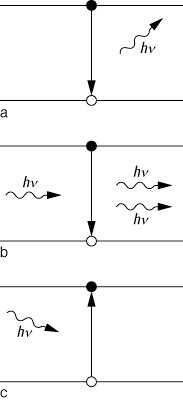
\includegraphics[width=0.2\textwidth]{emission.jpg}
\caption{Laserprinzipien: a) spontane Emission; b) induzierte Emission; c) Absorption.\cite{spektrum}}
\label{fig:emission}
\end{figure}

Findet nun mehr stimulierte Emission statt als Absorption, dann wird immer mehr Licht in Richtung des
bereits vorhandenen Lichts emittiert und das Licht wird immer weiter verstärkt. Dazu müssen sich allerdings mehr Atome im
angeregten als im nicht-angeregten Zustand befinden, da beide Prozesse gleich wahrscheinlich sind. Dieser Zustand wird
Besetzungsinversion genannt.
Er bedeutet jedoch eine Abweichung vom thermodynamischen Gleichgewicht. In diesem befinden sich nämlich mehr Atome im nicht-angeregten
Zustand. Aus diesem Grund muss dem Medium durch sogenanntes Pumpen Energie zugeführt werden.

\begin{figure}
\centering
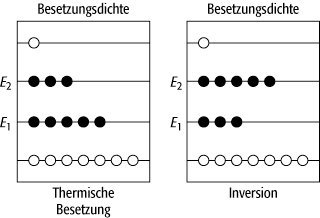
\includegraphics[width=0.4\textwidth]{inversion.jpg}
\caption{Besetzungsdichte bei Inversion im Vergleich zur thermischen Besetzung.\cite{spektrum}}
\label{fig:inversion}
\end{figure}

\subsection{Die Energiepumpe}

Im Glasrohr des Resonators befinden sich zwei Elektroden, an die eine Spannung angelegt wird. Dadurch kommt es im Lasermedium
zur Gasentladung, welche die Heliumatome in einen angeregten Zustand bringt. Durch Stöße übertragen die Heliumatome dann
ihre Energie auf die Neonatome und erzeugen so eine Besetzungsinversion zwischen energetisch hohen und niedrigen
Zuständen.

Das Medium im Laser muss dabei mindstens drei verschiedene Niveaus besetzen können, da in einem 2-Niveau-Laser keine
Besetzungsinversion möglich ist.

\subsection{Die TEM-Moden}

Im Laser sind verschiedene Moden realisierbar, da die Resonanzbedingung $L = n*\lambda/2$ des Resonators von mehreren Wellenlängen
erfüllt werden kann. Die Moden werden dabei als TEM-Moden (Transverse Electromagnetic Modes) bezeichnet. Zwei Zahlen
im Index geben die Ordnung der Moden in x- bzw. y-Richtung an.

Die Intensität der Moden in der einfachsten Ordnung 00 wird durch eine Gaußverteilung beschrieben:

\begin{equation}
  I_{00} = I_0 \text{exp} \biggl(\frac{-2r^2}{\omega^2}\biggr)
\end{equation}

Im He-Ne-Laser mit Brewsterfenstern gilt für alle höheren Ordnungen:

\begin{equation}
  I_{mn} = I_0 \biggl(\frac{\omega_0}{\omega}\biggr)^2 \biggl\lbrack H_m \biggl( \frac{\sqrt(2)x}{\omega} \biggr) \text{exp} \biggl( \frac{-x^2}{\omega^2} \biggr) \biggr\rbrack^2 \biggl\lbrack H_n \biggl( \frac{\sqrt(2)y}{\omega} \biggr) \text{exp} \biggl( \frac{-y^2}{\omega^2} \biggr) \biggr\rbrack^2
\end{equation}

($H$: Hermitesches Polynom, $\omega$: Strahlradius, $\omega_0$: kleinster Strahlradius)

\subsection{Intensität des polarisierten Lichts}

Die Intensität des Lichtes hinter einem Polarisationsfilter lässt sich durch die folgende Formel betimmen.

\begin{equation}
  I = I_0 \text{cos}^2(\delta\phi)
\label{eq:pol}
\end{equation}

Dabei ist $I_0$ die Intensität des Lichtes vor dem Filter und $\delta\phi$ der zur Einstellung des Filters verschobene Winkel
der Polarisation des einfallenden Lichtes.

\subsection{Die Wellenlänge des Lasers}

Die Wellenlänge des Lichts wird gemessen, indem ein Gitter in den Strahl gebracht wird. Auf diese Weise treten Interferenzeffekte
auf einem Schirm auf. Mit Hilfe des Abstandes $x$ zwischen dem 0. und dem 1. Hauptmaximum kann die Wellenlänge berechnet werden.

\begin{equation}
  \lambda = g \text{sin}(\text{arctan}(x/d))
\label{eq:wellen}
\end{equation}

Dabei ist $d$ der Abstand zwischen Schirm und Gitter und $g$ die Gitterkonstante.
